\documentclass[]{article}
\usepackage[pdftex,paperwidth=434pt,paperheight=316pt,noheadfoot,left=0pt,top=0pt]{geometry}
\usepackage{graphicx}

\begin{document}
\noindent
%\scalebox{0.8819}[0.8966]{
\begin{picture}(432,315)
\put(-108,-254){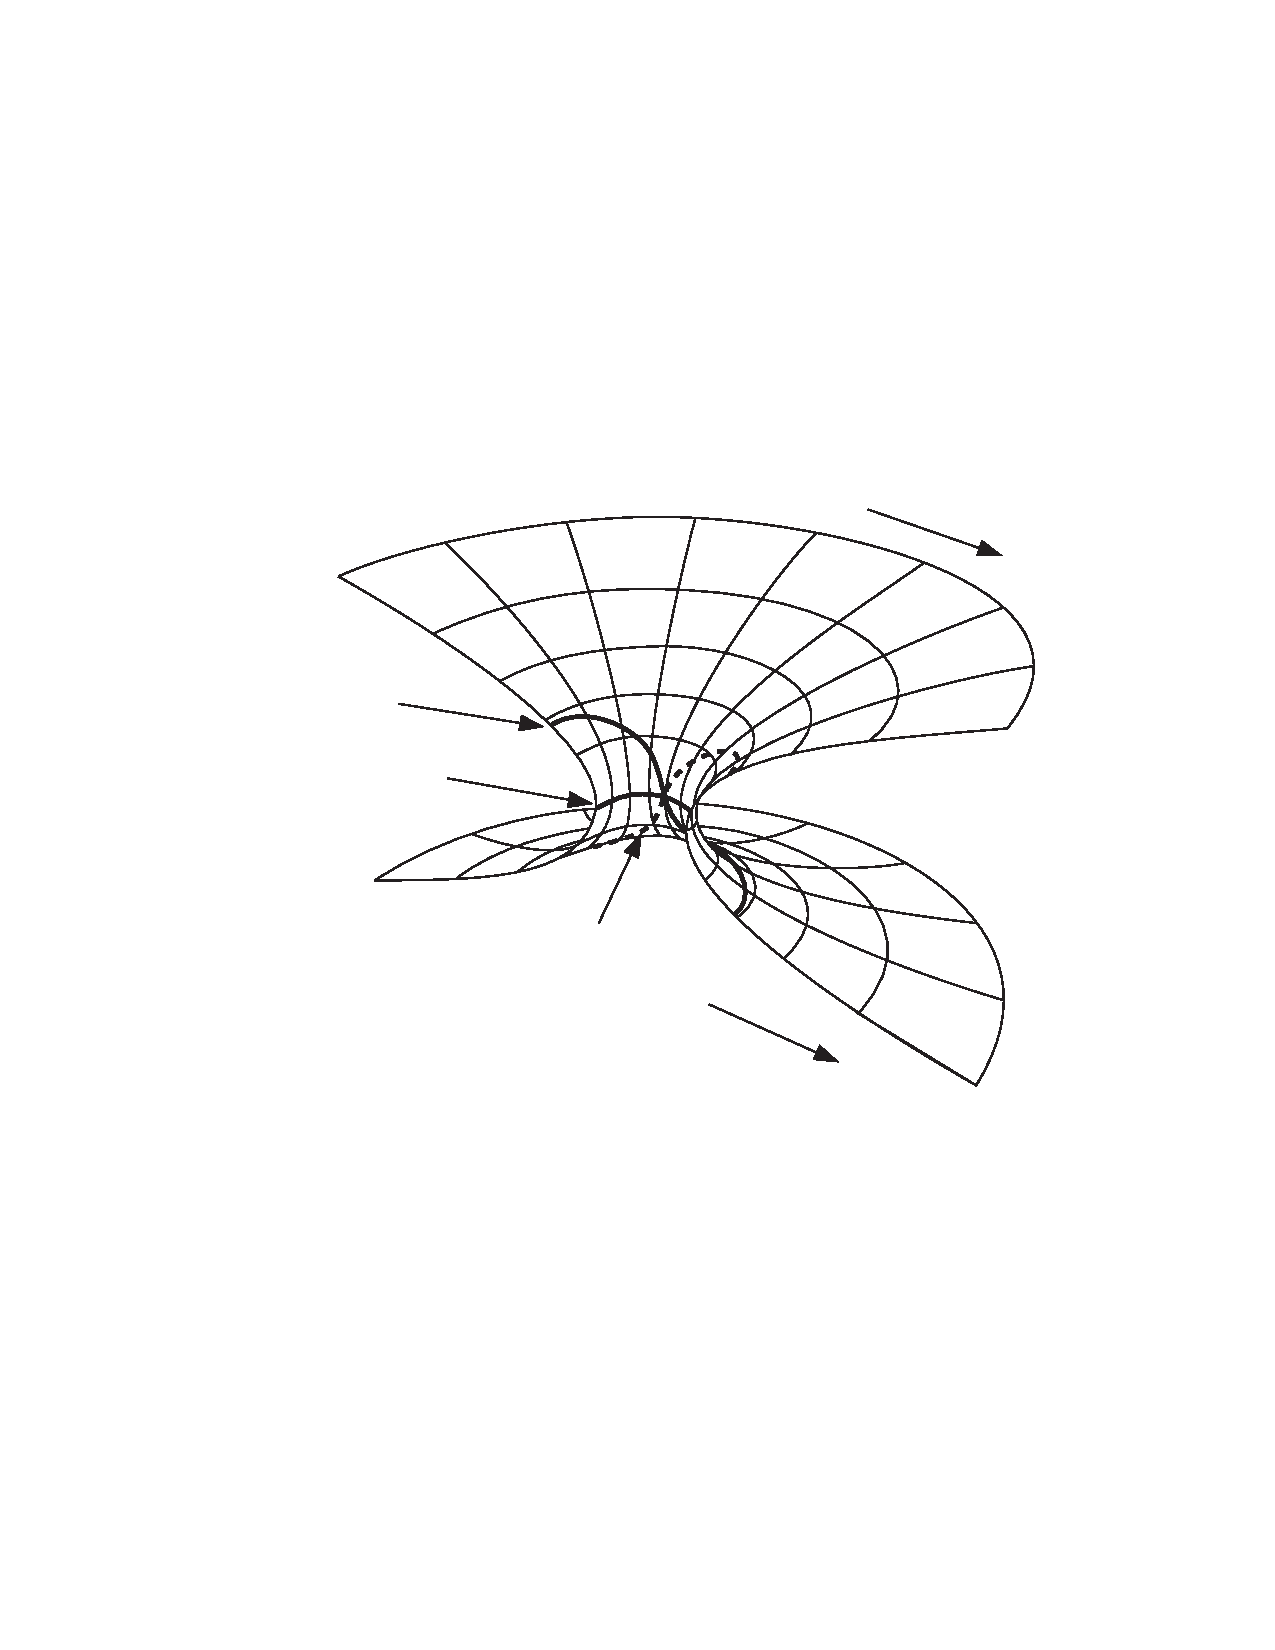
\includegraphics[width=8.5in]{PDFnotext/Figure13_5.pdf}}
\put(348,287){\boldmath{P}}
\put(257,33){\boldmath{P}}
\put(383,183){$\theta=0$}
\put(22,260){$\theta=\pi$}
\put(31,198){Top Sheet}
\put(31,188){Apparent Horizon}
\put(111,94){Bottom Sheet}
\put(111,84){Apparent Horizon}
\put(58,163){Minimal}
\put(58,153){Surface}
\end{picture}
%}
\end{document}
